%--------------------------------------------------------------------
% \chapter{Sensor Collection Service}
%--------------------------------------------------------------------

% Problems with earlier implementation:
% 1. Bad performance in field trial. Irregularities in data
% 2. Not cross platform

% Improved Sensor Collection Architecture:
% * Performance improvements
% * Better exchange format
% * Simpler design / Extendability
% * Improved Data Inspection Front End
% * More Flexibility to add HAR as a service
% * Integration into Service Center
% * Removed dependency on external lib


% In particular cover the topics:
% \begin{enumerate}
% \item Improved Architecture Description
% \item Inspection Front End
% \item New Sensor Transfer File Format
% \item New Streaming API
% \item Integration Loging and Heartbeating into Upload Servlet
% \item Data Collection event in Koblenz
% \end{enumerate}


\section{Mobile Sensor Collector}

The revised sensor collector follows the following architecture
(Figure \ref{fig:sc_architecture}).

\begin{figure}[htbp]
\centering
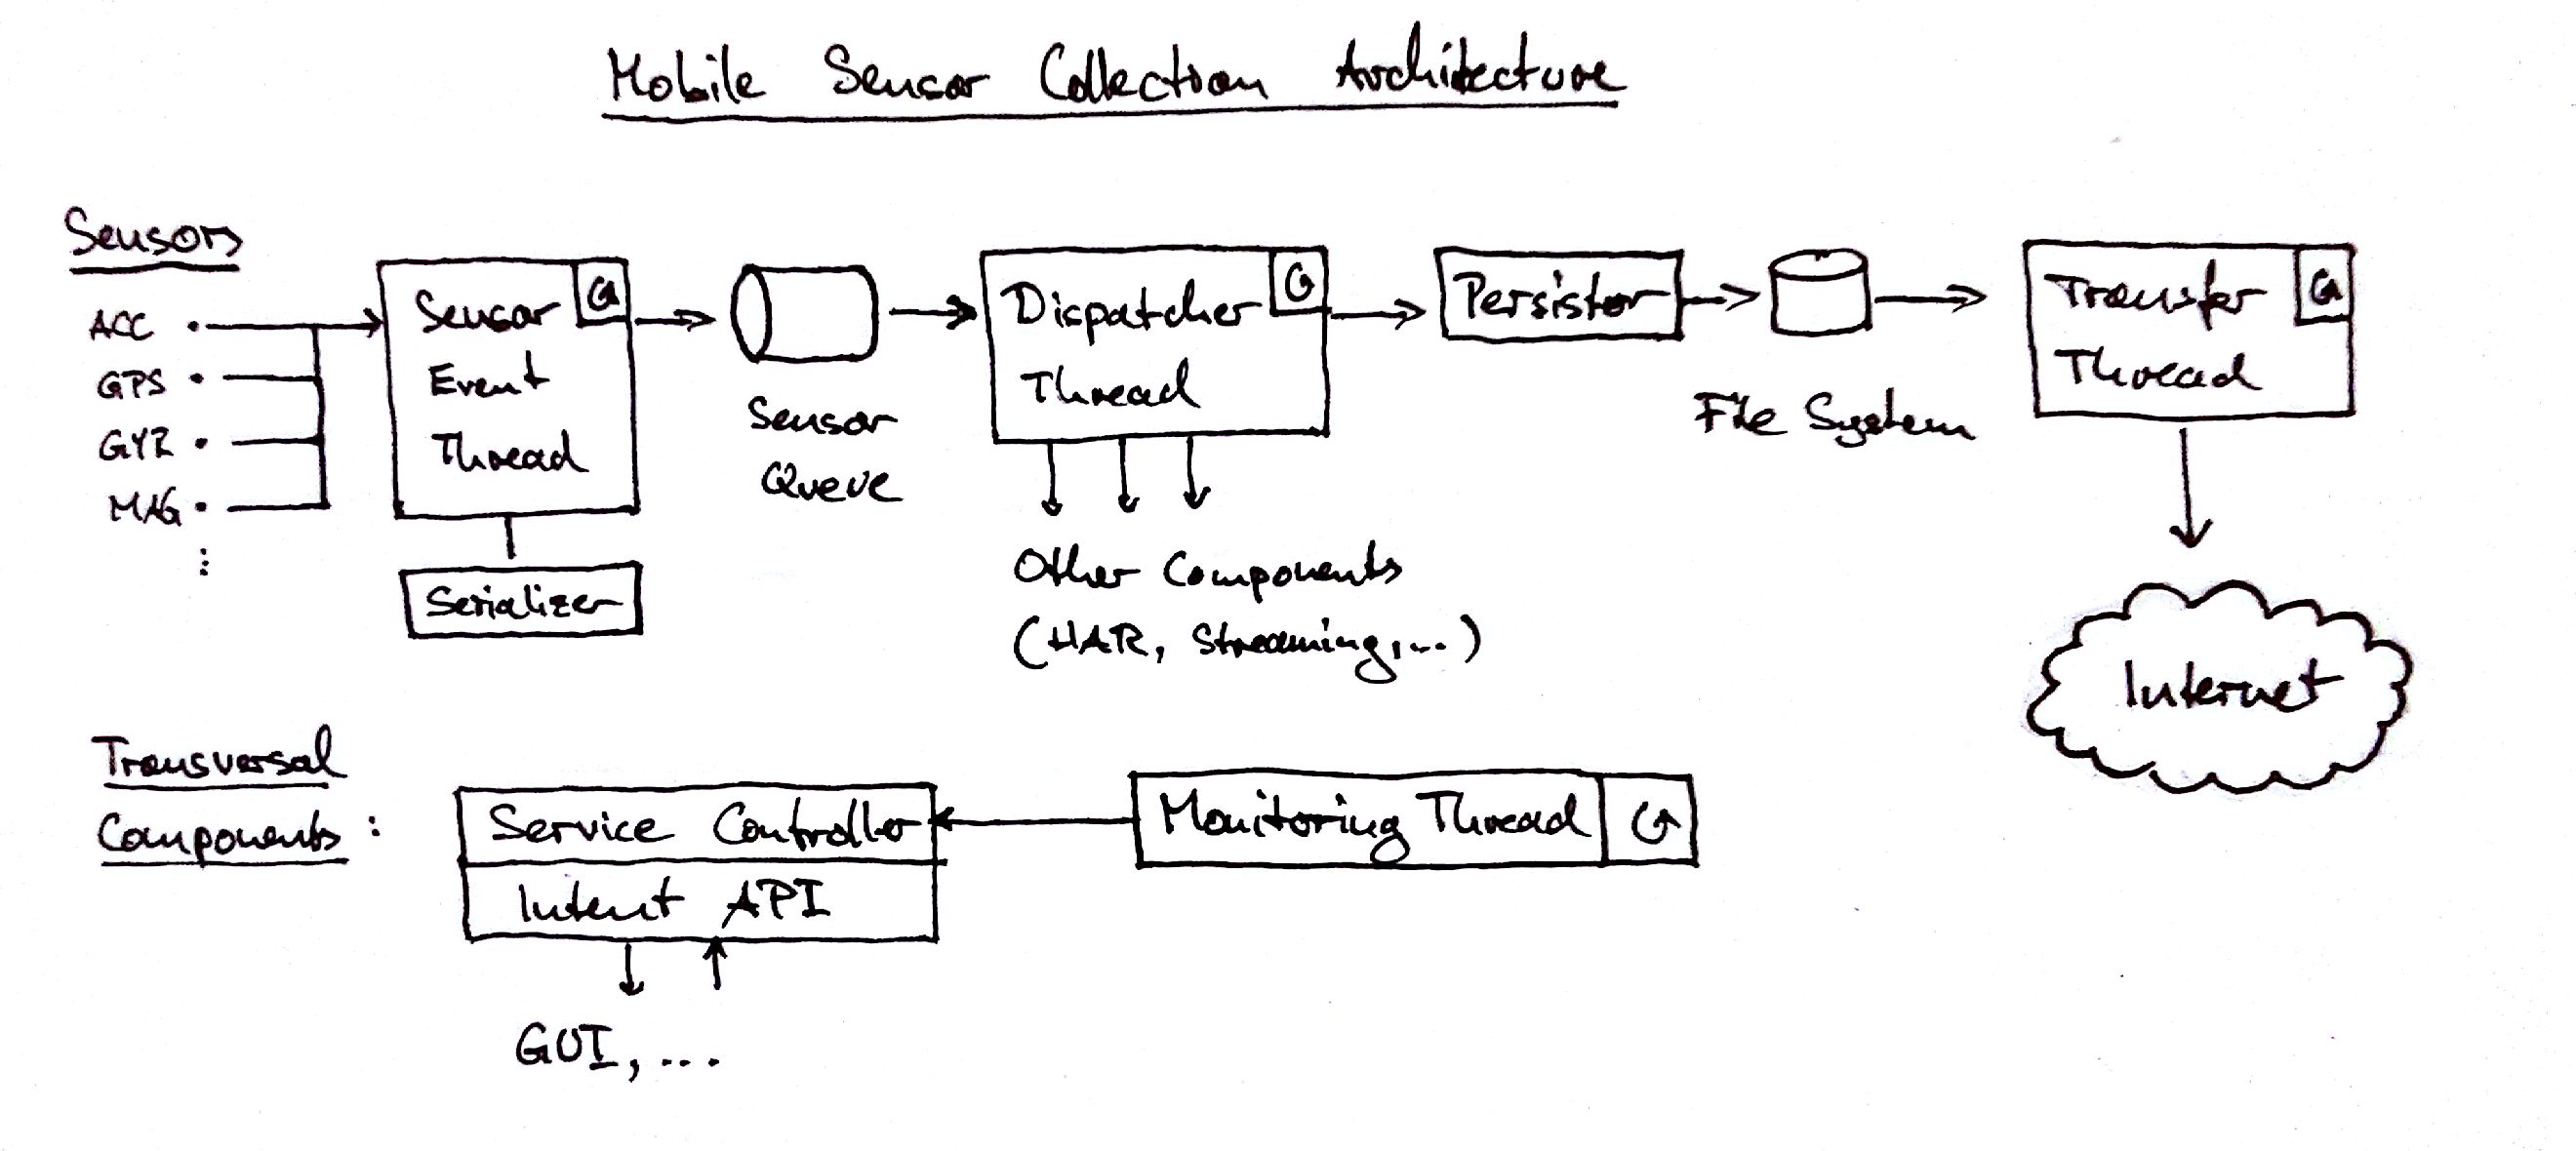
\includegraphics[width=\textwidth]{img/sc/sc_architecture.jpg}
\caption{Sensor Collection Architecture}\label{fig:sc_architecture}
\end{figure}

The architecture consists of the following components:
\begin{itemize}
\item {\bf Sensor Event Thread}. The sensor event thread registers
  callback listeners for all configured sensors. When sensor events
  occur the received values are serialized in the ssf
  format (cf. \ref{sec:ssf}) and pushed onto the SensorQueue.
\item {\bf SensorQueue}. The sensor queue is a synchronized queue
  object that stores sensor values as strings.
\item {\bf DispatcherThread}. The dispatcher thread reads sensor
  values from the sensor queue and passes them to several services
  that can be registered. Included services are the persistor service
  and the activity recognition component, the streaming service and GPS
  publication pipeline (for use in the Service Line Detection API).
\item {\bf Persistor}. The persistor service is executed by the
  DispatcherThread and appends the received sensor sample into a
  predefined file. Also a variant with zip-file compression is
  included.
\item {\bf TransferThread}. The transfer thread is an independent
  thread that transfers the persisted samples to the Live+Gov Servers.
\item {\bf Monitoring Thread}. The monitoring thread polls the
  different components and gathers run-time information like numbers of
  processed samples or transfer state.
\item {\bf Service Controller}. The service controller starts and
  stops all running threads, and takes care of proper configuration of
  all services. It listens to Intents specified in the API and changes
  the state of the service accordingly.
\end{itemize}

The following table summarizes all supported sensors:

\begin{table}[ht]
\centering
\begin{tabular}{|l|p{0.7\linewidth}|}
  \hline
  Sensor & Description \\
  \hline
  GPS                 & Global position in latitude and longitude. 

                        If available, the GPS samples are gathered via
                        Google's new Play Services location
                        provider\footnote{https://developer.android.com/google/play-services/location.html}.
                        The advantages of this library for our use case are: the instant
                        availability of the last known location and a significant decrease
                        of power consumption, since several location providers (e.g. using
                        Wifi) are fused together.  
                        
                        If the Play Services are not available, the service falls back to
                        accessing the GPS samples directly.
  \\ \hline
  Accelerometer       & Measures the acceleration force in $m/s^2$
                        that is applied to a device on all three
                        physical axes. 

                        Also the low-pass and high-pass filtered
                        variants 'Linear Acceleration' and 'Gravity' offered by the Google
                        API can be captured.
  \\ 
  Rotation Vector     & Measures the orientation of a device by
                        providing the three elements of the device's
                        rotation vector.  
  \\
  Gyroscope           & Measures a device's rate of rotation in
                        $rad/s$ around each of the three physical
                        axes. 
  \\ 
  Magnetic field      & Measures the ambient geomagnetic field for all
                        three physical axes in $\mu T$. 
  \\ \hline
  WLAN                & A list of all available wireless local area
                        networks in the transmission range. 
  \\
  Bluetooth           & A list of all available bluetooth clients in
                        the transmission range. 
  \\
  GSM                 & Cellular network operator and the radio cell
                        the mobile phone is connected with. 
  \\ \hline
  Google Activity     & Google recently released an Activity
                        Recognition Library. The sensor collector is able to record activities as sensor
                        values as well. 
  \\
  \hline
\end{tabular}
\caption{Sensors recorded in the Live+Gov sensor collection app}
\label{SensorsOfLGCollectionApp}
\end{table}

\subsection{Intent API}


\label{subsubsec:IntentAPIdescription}

The communication with other Live+Gov toolkit components is
facilitated through the exchange intent
messages\footnote{\url{http://developer.android.com/guide/components/intents-filters.html}}. 
The API was slightly improved since deliverable D1.1. New intents are
marked with an asterisk (*).

The following API-calls are implemented.
\begin{itemize}
\item {\bfseries Start/Stop Service.} Starts and stops the sensor
  collector service. Samples can only be recorded, or transmitted when
  the service is running.
\item {\bfseries Start/Stop Recording.} Starts and stops recording of
  sensor samples.
\item {\bf Send Annotation.} This intent allows users to annotate
  their recording by a string value that will be recorded by a
  ``tag-sensor''.
\item {\bfseries Enable/Disable sample storage.} Samples are stored in
  a local database, of variable size. If Disabled samples can still be
  broadcasted to the system.
\item {\bfseries Enable/Disable continues sample transfer.} Controls
  the sample transfer state machine. When enabled and a network
  connection is available sensor samples are transfered in batches to
  the server backend.
\item {\bfseries Transfer samples.} Triggers the sample transfer.
\item {\bfseries Enable/Disable sample broadcast.} When enabled all
  recorded sensor samples are broadcasted in the form of intents into
  the system. This allows other components, e.g. feature extraction
  and context mining, to make use of the recorded sensor data.
\item {\bfseries Request Status Report.} When this intent is received
  a status report is broadcasted to the system.
\item {\bfseries Tag sample.}  Annotations by users are realized as
  ``Tag sample''.  The content of this intents is included as
  ``tag''-sensor in the recording.
\end{itemize}

When a control intent is received by the component, the appropriate
action is taken. After execution has finished a status report intent
is broadcasted to the system which provides information about whether
the requested method call was successful (cf. Table
\ref{tab:StatusIntent}).  Further technical description of the
component and the API are included in D4.1.

% Status intents contain the following information:
\begin{table}[ht]
\centering
\begin{tabular}{|l|l|l|} \hline
   Key       & Type    & Description                                       \\ \hline
   running   & boolean & True if service is running.                       \\
   recording & boolean & True if sensor samples are recorded.              \\
   storage   & boolean & True if samples are stored in the database.       \\
   transfer  & boolean & True if continues transfer of samples is enabled. \\
   broadcast & boolean & True if samples are broadcasted.                  \\ \hline
\end{tabular}
\caption{Structure of status intents}
\label{tab:StatusIntent}
\end{table}

The sensor sample broadcast intent contains a unique device
identifier, a timestamp and serialized sample data in XML
format. Figure \ref{fig:XMLSamples} shows two examples for GPS and
accelerometer samples.

\subsection{Testing GUI}

\begin{figure}[htbp]
\centering
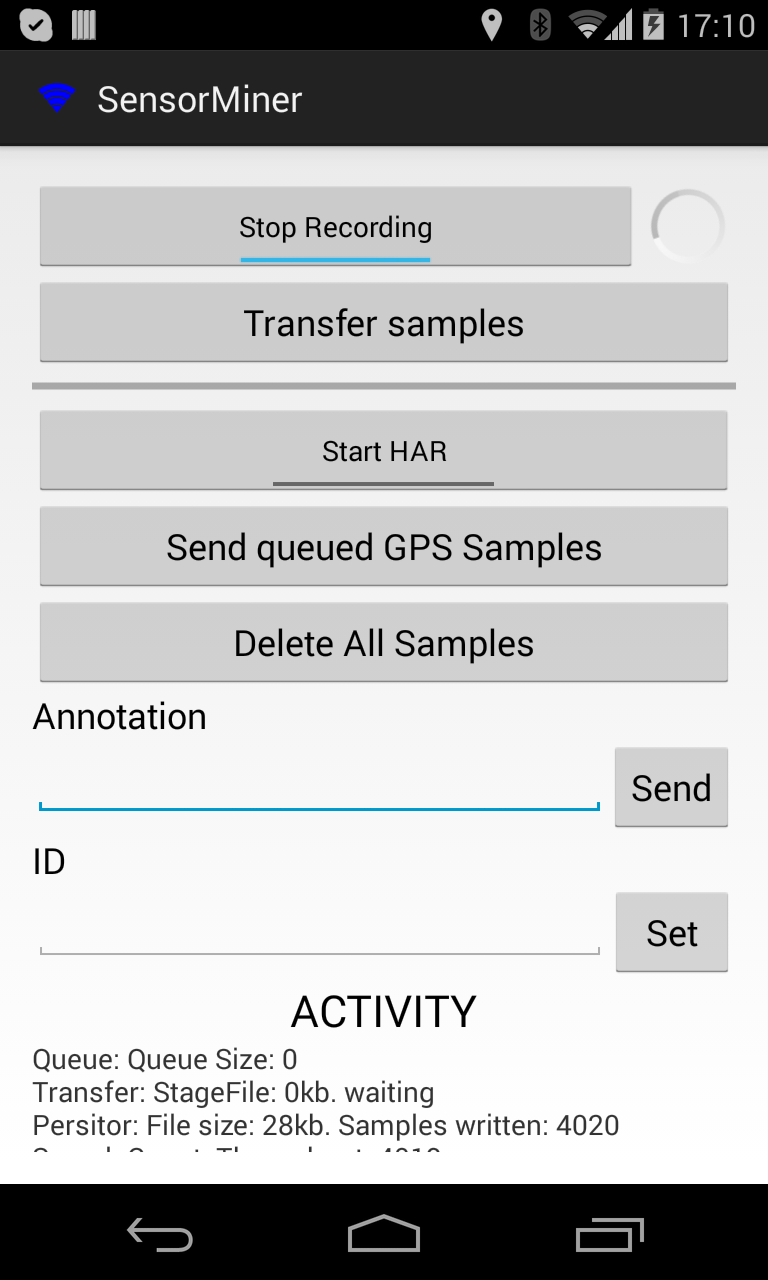
\includegraphics[width=0.3 \textwidth]{img/sc/sc_gui.png}
\caption{Sensor Collection Architecture}\label{fig:sc_gui}
\end{figure}

\subsection{Sensor Stream File Format}\label{sec:ssf}
This document describes the sensor stream format ({\it ssf}) which is used for
transfering sensor values from a mobile device (or another sensor
source) to the Live+Gov data-base. The file format is inspired by the
\href{http://en.wikipedia.org/wiki/Common\_Log\_Format}{Common Log
  Format} used by many webservers. We view incoming sensor values as
events and record them as a simple stream of CSV-rows. Each sensor has
an individual prefix but writes into the same file.

The key advantages of this format as opposed to the previously used
XML format are:
\begin{itemize}
\item Human readability. The format is easy to understand by humans.
\item Statelessness. Every line can be interpreted without the context
  of the file. Therefore ssf-files can be arbitrarily sliced,
  concatenated and filtered using UNIX tools like {\it grep, cat, sed,
    awk}.
\item Streaming. Lines can be individually transferred over tcp
  sockets or messaging systems. Allowing immediate inspection of the
  recorded samples on a remote system.
\end{itemize}

\subsubsection*{Format Description}

The rows of the ssf-format have the following structure:
\small
\begin{verbatim}
SENSOR_PREFIX,TIME_STAMP, USER_ID, SENSOR_VALUES
\end{verbatim}
\normalsize


The authorative source for the field descriptions is the source code.

\begin{itemize}
\item \texttt{SENSOR PREFIX}. Identifies the sensor producing the
  sample. The following sensor prefixes are supported: \\
  \texttt{GPS} (GPS sensor), \texttt{ACC} (Accelerometer),
  \texttt{LAC} (Linear Acceleration), \texttt{GRA} (Gravity),
  \texttt{GYR} (Gyroscope), \texttt{MAG} (Magnetometer), \texttt{WIFI}
  (Wifi networks), \texttt{BLT} (Bluetooth), \texttt{GSM} (GSM cells),
  \texttt{ACT} (Google Play Services Activity), \texttt{ERR} (Error
  Value), \texttt{TAG} (Annotations entered by the user).
\item \texttt{TIME STAMP} UNIX timestamp in milliseconds e.g. \texttt{1377609577214}
\item \texttt{USER ID} ID that identifies records from the same
  user. The default value is the device-id that is provided by
  Android.
\item \texttt{SENSOR VALUES} 
  Sensor values in individual formats. In order to adhere to the CSV
  standard no \texttt{,}-symbol and new-lines may be used in this field.
  \begin{itemize}
  \item \texttt{ACC/GYR/MAG/LAC/GRA} X,Y,Z-values separated by space characters.
  \item \texttt{GPS} lat,lon,alt-values separated by space characters
  \item \texttt{ACT} Activity Name, Confidence separated by space characters.
  \item \texttt{WIFI} List of access-points, where each visible
    accesspoint is separated by a \texttt{;} and written as

    Escaped SSID String/Escaped BSSID String/Frequency in MHz/RSSI in dBm
  \item \texttt{BLT}
    List of devices where each visible device is separated by a \texttt{;}
    and written as
    Escaped Address/Device Major Class/Device Class/Bond
    State/Optional Escaped Name/Optional RSSI
  \item \texttt{GSM}
    The state of the device written as Service State/Roaming State/Manual
    Carrier Selection State/Escaped Carrier Name/Escaped Signal Strength

    followed by \texttt{:}, followed by a possibly empty list of cells,
    where each cell is separated by a \texttt{;} and written as
    Escaped Cell Identity/Cell Type/RSSI in dBm
  \end{itemize}
\end{itemize}

Example rows may look as follows:
\small
\begin{verbatim}
ACC,1377605748123,5,0.9813749 0.0021324 0.0142523
GPS,1377605748156,5,50.32124 25.2453 136.5335
WIFI,1341244415,wifiUser,"WiFi AP"/"00:12:42"/2412/-45; "Another WiFi AP"/"33:13:53"/2437/-56
TAG,1378114981049,anotherUser,"test tag"
BLT,1385988380374,bluetoothUser,"C8:F7:33:B7:B5:B4"/computer/computer laptop/bonded/"LAPTOP"/-46
\end{verbatim}
\normalsize

\subsection{Streaming Service}

The revised version of the sensor collector includes a streaming
service, that transfers recorded samples directly to a remote machine.

The streaming service uses the ZeroMQ networking
library\footnote{http://www.zeromq.org} to transfer single ssf lines
to the Live+Gov machine running a streaming server. The streaming
server appends the received samples to a file (zmq\_stream.ssf).

This simple service allows direct monitoring of the recorded samples,
via simple UNIX command line tools, e.g. 
\begin{verbatim} 
tail -f zmq_stream.ssf 
\end{verbatim}
prints the recoded samples to the console.
\begin{verbatim} 
tail -f zmq_stream.ssf | grep ^GPS 
\end{verbatim} 
filters out gps samples. And finally
\begin{verbatim} 
tail -f zmq_stream.ssh | cut --delimiter=',' --field=1 | logtop  
\end{verbatim}

shows the frequencies of the individual incoming sensor values.

\section{Sensor Storage Service Architecture}

\begin{figure}[htbp]
\centering
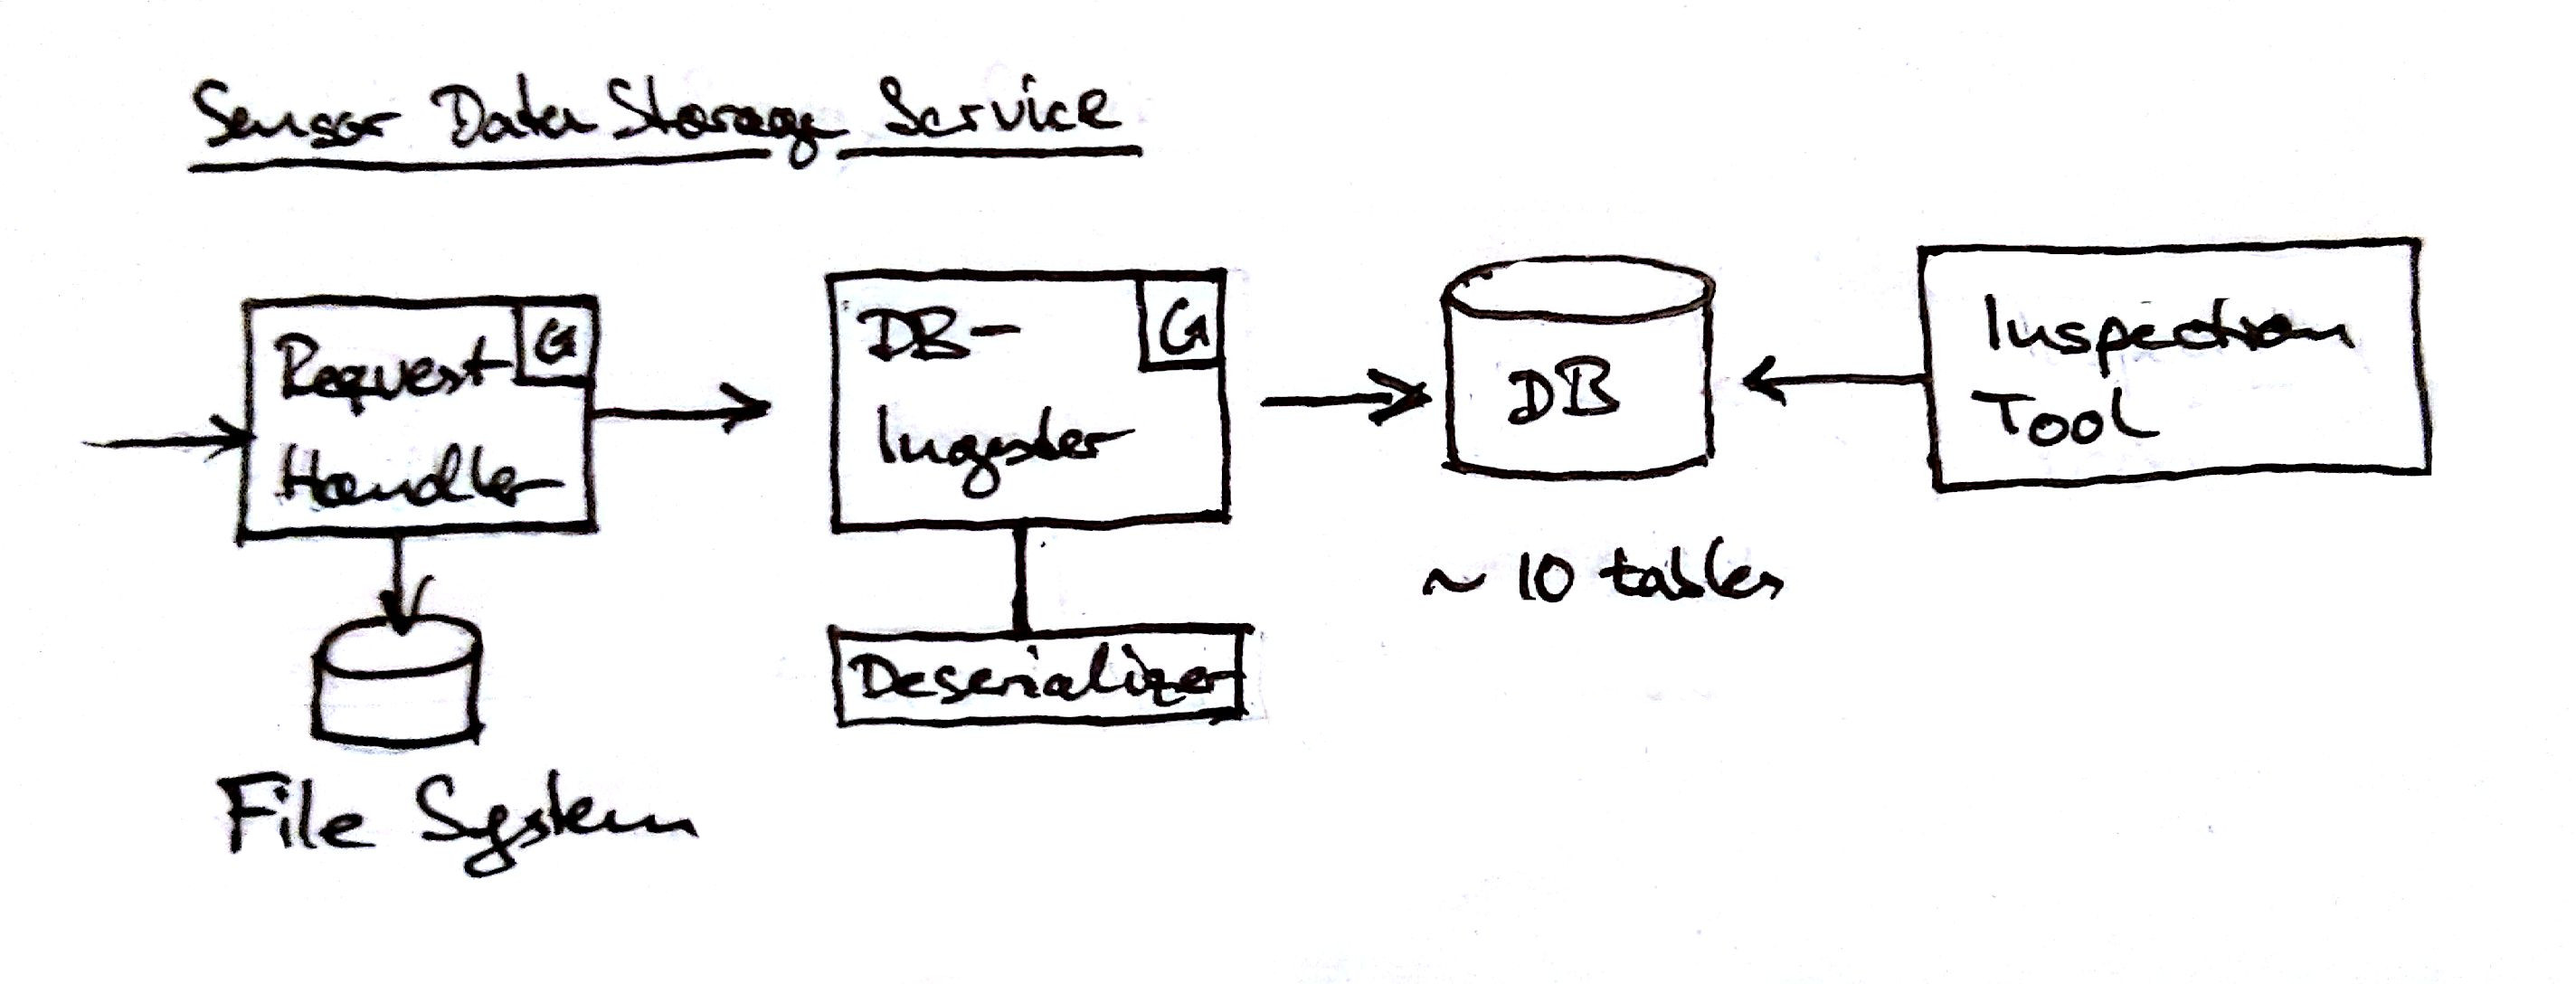
\includegraphics[width=0.7\textwidth]{img/sc/ss_architecture.jpg}
\caption{Sensor Collection Architecture}\label{fig:ss_architecture}
\end{figure}

Architecture Description

\subsection{Database Scheme}

The uploaded samples are stored in a
PostgreSQL\footnote{http://www.postgresql.org/} database. We have
switched from MySQL to this technology, because of the advanced query
fuctionality that is offered by the
PostGIS\footnote{http://postgis.net/} plugin.

The database has the following schema:
{\small
\begin{verbatim}
sensor_gps (trip_id INT, ts BIGINT, lonlat GEOGRAPHY(Point));
sensor_accelerometer (trip_id INT, ts BIGINT, x FLOAT, y FLOAT, z FLOAT);
sensor_linear_acceleration (trip_id INT, ts BIGINT, x FLOAT, y FLOAT, z FLOAT);
sensor_gravity (trip_id INT, ts BIGINT, x FLOAT, y FLOAT, z FLOAT);
sensor_tags (trip_id INT, ts BIGINT, tag TEXT);
sensor_google_activity (trip_id INT, ts BIGINT, activity TEXT);
har_annotation (trip_id INT, ts BIGINT, tag TEXT);
\end{verbatim}}

\subsection{Inspection Front End}


\subsection{Integration of Logging and Heartbeats}



\subsection{Cross-Platform Strategy}
Explain problems with Titanium framework.

Android component runs on Blackberry. 

Implement HAR as SAAS. Write client app for iOS.


%%% Local Variables:
%%% mode: latex
%%% TeX-master: "../D1-2"
%%% End:
